\documentclass{beamer}
\usepackage{mathpazo}
\usepackage[latin1]{inputenc}
\usepackage[cyr]{aeguill}
\usepackage[francais]{babel}
\usepackage[T1]{fontenc}


\usepackage{epstopdf} 
\usepackage{caption}
\usepackage{subcaption}


\usetheme{ENSLyon} 
\title[Title]{Une m�thode de calibration non param�trique pour les calorim�tres de CMS}
\author[Samuel Niang]{Samuel Niang}
\date{\today}
  \setbeamersize{text margin left=0mm}
  \setbeamersize{text margin right=0mm}


% pour supprimer les symboles de navigation
\setbeamertemplate{navigation symbols}{}
\usecolortheme{ENSLyon_blue}


\begin{document}



\begin{frame}
	\titlepage
	\begin{center}
            	\includegraphics[height=1cm]{images/Logo_IPNL.jpg} 
            	\hspace{1cm}
            	\includegraphics[height=1cm]{images/Logo_CMS.png} 
		\hspace{1cm}
	 	
\includegraphics[height=1cm]{images/logoens.eps}
		\hspace{1cm}
		\includegraphics[height=1cm]{images/logoucbl.eps}
        \end{center}
\end{frame}


\section{Introduction}
\subsection{Contexte}
\begin{frame}{D�tecteur}
\begin{figure}[!h]
\begin{center}
\includegraphics[height=0.7\textheight]{images/detecteur.pdf}
\caption{Une esquisse des interactions sp�cifiques des particules dans une tranche transversale du d�tecteur CMS.}
\label{detecteur}
\end{center}
\end{figure}
\end{frame}

\subsection{Production de l'�chantillon}
\begin{frame}{Illustration de particules simul�es}
\begin{figure}[!h]
\begin{center}
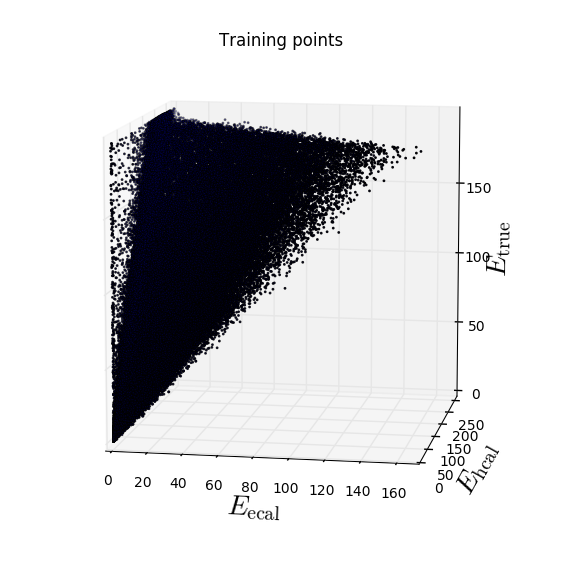
\includegraphics[height=0.7\textheight]{images/pictures/testLinearRegression/LinearRegression_plot3D_training.png}
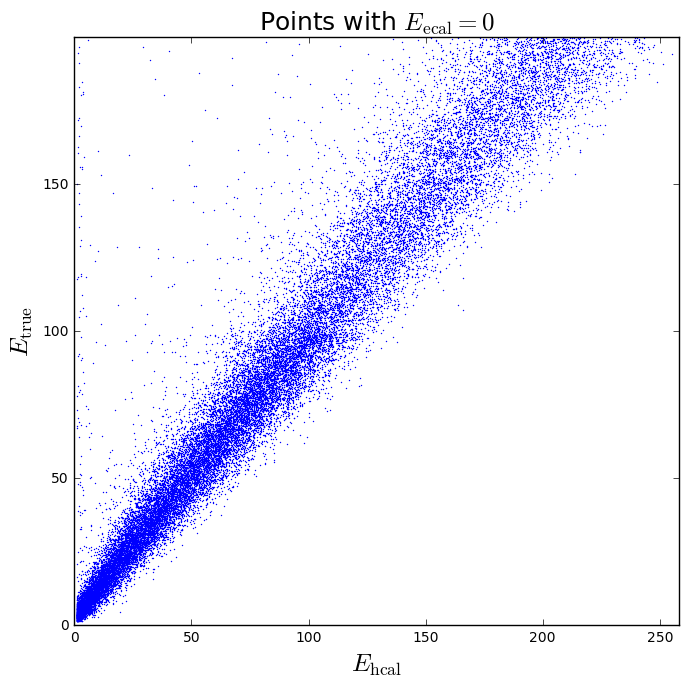
\includegraphics[height=0.7\textheight]{images/pictures/explain/ecal_eq_0.png}
\caption{\'Energie vraie $E_{\rm true}$ en fonction de l'�nergie mesur�e dans le ECAL, $E_{\rm ecal} \neq 0$, et de l'�nergie mesur�e dans le HCAL.}
\label{points}
\end{center}
\end{figure}
\end{frame}

\section{M�thodes de calibrations propos�es}

\subsection{Calibration par r�gression lin�aire}
\begin{frame}{Issues and objectives 1}

\end{frame}

\subsection{M�thode non param�trique bin�e}
\begin{frame}{Issues and objectives 1}

\end{frame}

\subsection{Moyenne pond�r�e}
\begin{frame}{Issues and objectives 1}

\end{frame}

\subsection{Nettoyage gaussien}
\begin{frame}{Issues and objectives 1}

\end{frame}

\subsection{Fit gaussien}
\begin{frame}{Issues and objectives 1}

\end{frame}

\section{Comparaison et r�sultats}
\begin{frame}{$E_{\rm calib}/E_{\rm true}$ moyens en fonction de $(E_{\rm ecal},E_{\rm hcal})$}
\begin{figure}
\begin{center}
\begin{subfigure}{0.31\textwidth}
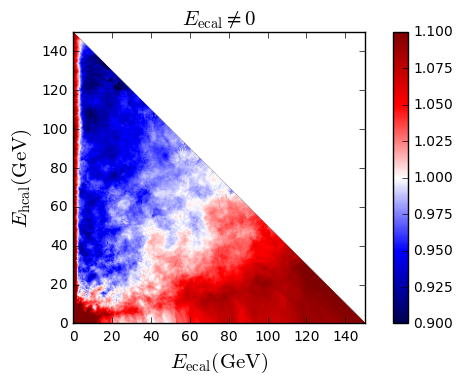
\includegraphics[width=\textwidth]{images/pictures/comparisons/ecaliboveretrue_LinearRegression.png}
\caption{R�gression lin�aire}
\end{subfigure}
\begin{subfigure}{0.31\textwidth}
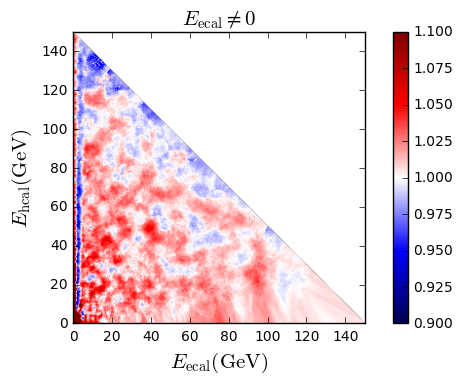
\includegraphics[width=\textwidth]{images/pictures/comparisons/ecaliboveretrue_CalibrationLego.png}
\caption{M�thode non param�trique bin�e}
\end{subfigure}
\begin{subfigure}{0.31\textwidth}
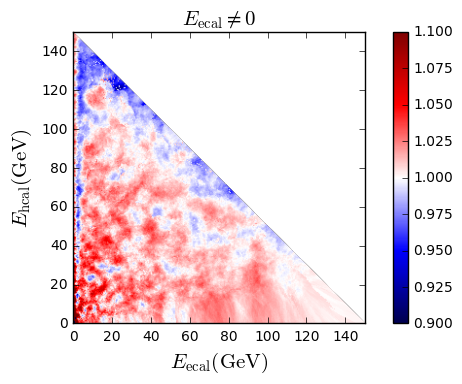
\includegraphics[width=\textwidth]{images/pictures/comparisons/ecaliboveretrue_KNN.png}
\caption{Plus proches voisins}
\end{subfigure}
\end{center}
\caption{Chaque pixel correspond � la moyenne d'un fit gaussien de points $E_{\rm calib}/E_{\rm true}$ proches des coordonn�es du pixel pour les particules qui interagissent avec le ECAL et le HCAL.}
\label{comparaison2}
\end{figure}
\end{frame}

\begin{frame}{$E_{\rm calib}/E_{\rm true}$ moyens en fonction de $(E_{\rm ecal},E_{\rm hcal})$}
\begin{figure}
\begin{center}
\begin{subfigure}{0.31\textwidth}
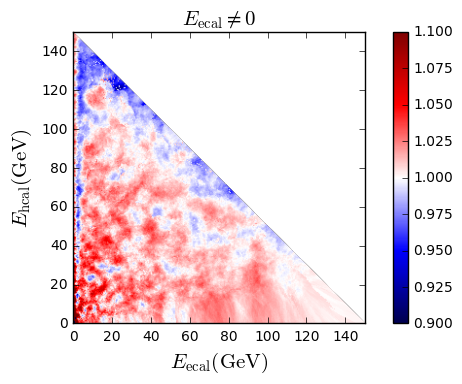
\includegraphics[width=\textwidth]{images/pictures/comparisons/ecaliboveretrue_KNN.png}
\caption{Plus proches voisins}
\end{subfigure}
\begin{subfigure}{0.31\textwidth}
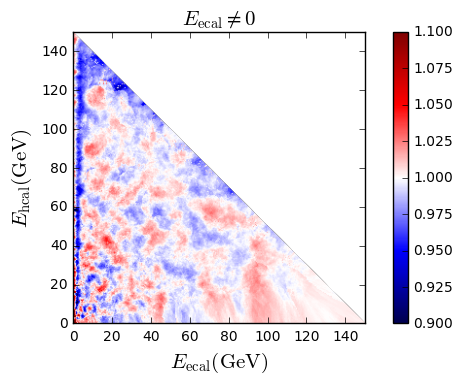
\includegraphics[width=\textwidth]{images/pictures/comparisons/ecaliboveretrue_KNNGaussianCleaning.png}
\caption{Plus proches voisins - Nettoyage gaussien}
\end{subfigure}
\begin{subfigure}{0.31\textwidth}
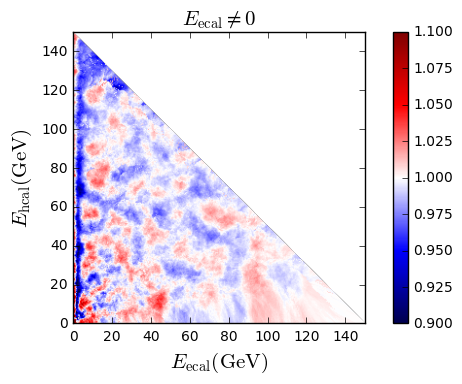
\includegraphics[width=\textwidth]{images/pictures/comparisons/ecaliboveretrue_KNNGaussianFit.png}
\caption{Plus proches voisins - Fit gaussien}
\end{subfigure}
\end{center}
\caption{Chaque pixel correspond � la moyenne d'un fit gaussien de points $E_{\rm calib}/E_{\rm true}$ proches des coordonn�es du pixel pour les particules qui interagissent avec le ECAL et le HCAL.}
\label{comparaison2}
\end{figure}
\end{frame}

\begin{frame}{$E_{\rm calib}/E_{\rm true}$ moyens en fonction de $E_{\rm true}$}
\begin{figure}[!h]
\centering
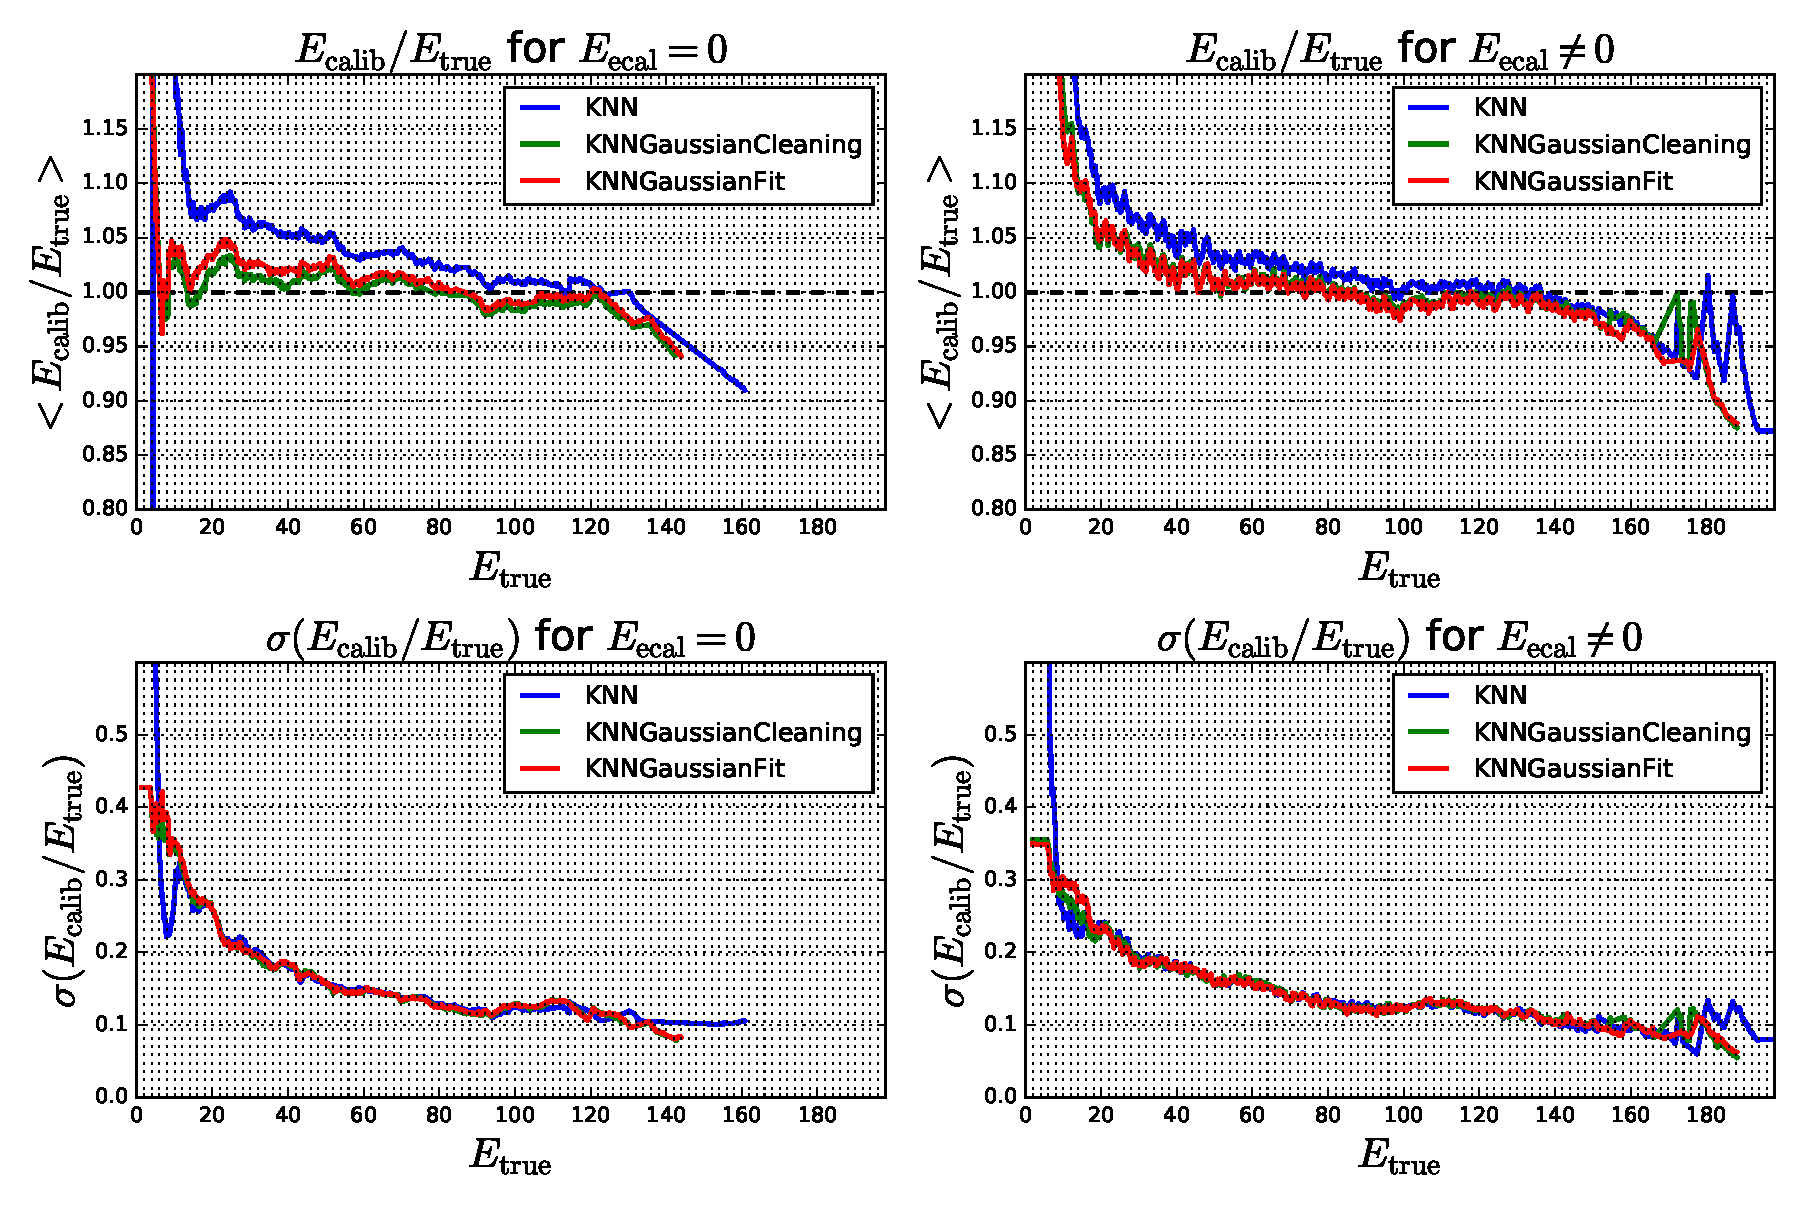
\includegraphics[height=0.75\textheight]{images/pictures/comparisons/comparison2.eps}
\caption{$E_{\rm calib}/E_{\rm true}$ moyens en fonction de $E_{\rm true}$ dans les cas $E_{\rm ecal} = 0$et $\sigma$ du fit gaussien correspondant.}
\label{comparaison3}
\end{figure}
\end{frame}


\section{Conclusion}
\begin{frame}{Conclusion}

\end{frame}

\end{document}
